\begin{center}
\begin{minipage}{0.7\textwidth}
    \centering
    \fbox{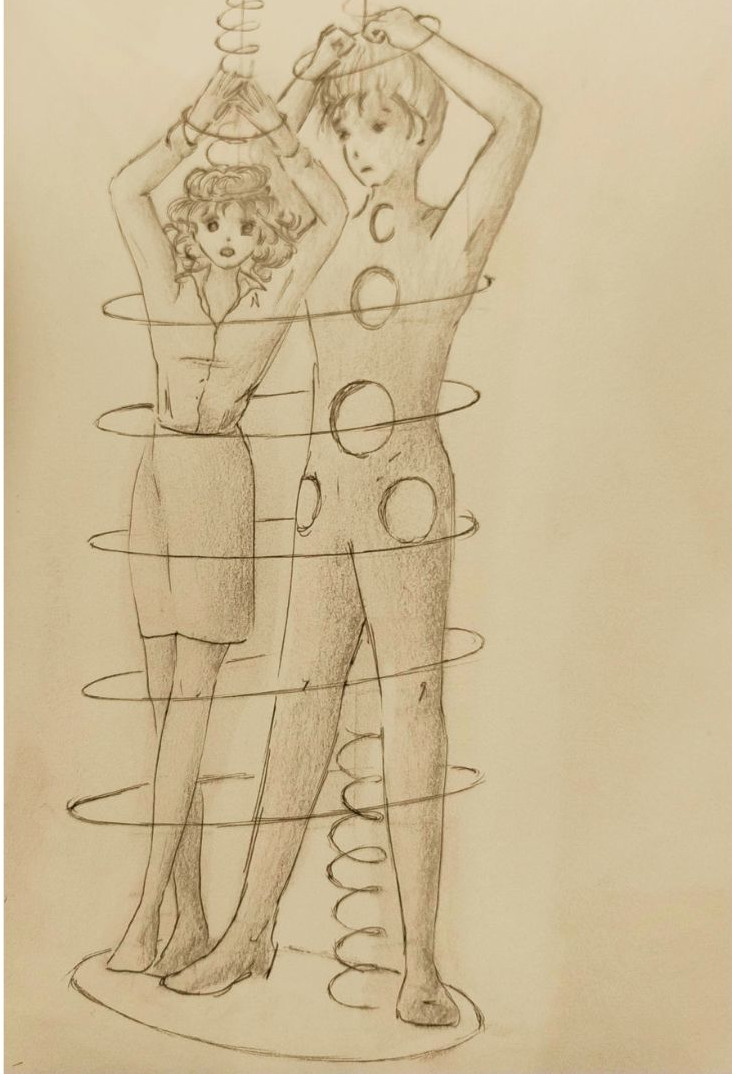
\includegraphics[width=\textwidth]{immagini/cnot_100.jpeg}} % Sostituisci con il nome del file immagine
\end{minipage}
\end{center}


\begin{tcolorbox}[colback=gray!5,colframe=gray!80,title=\textbf{Scheda Informativa}]
\begin{itemize}
    \item \textbf{Luogo}: CCU (Classical Control Unit)
    \item \textbf{Giorno e ora}: Il tempo non è osservabile
    \item \textbf{Situazione}: Caterina è stata arrestata.
\end{itemize}
\end{tcolorbox}



\vspace{1em}
\begin{center}Caterina\end{center}
\hrule
\vspace{1em}

Mi trovavo in una stanza spoglia, con pareti metalliche che riflettevano una luce bianca e fredda. La mia mente era in tumulto: la paura mi attanagliava, la confusione mi annebbiava i pensieri, e un desiderio disperato di fuggire cresceva dentro di me. Di fronte a me si stagliava il Supervisore, una figura imponente dai tratti austeri e rigidi, che mi fissava con uno sguardo duro e indagatore. Sentivo il cuore battere all'impazzata, e percepivo chiaramente la tensione che emanava, quasi come se quel controllo assoluto che cercava di mantenere nascondesse qualcosa di fragile.

Accanto a me c'erano Mark e l'altro compagno, anch'essi in attesa, immobili e silenziosi. Gli agenti che ci avevano catturato si erano ritirati, lasciandoci soli con il Supervisore. Sentivo il respiro regolare di Mark al mio fianco; la sua presenza mi dava conforto, ma non riusciva a placare l'ansia che cresceva dentro di me. Mi sentivo così piccola e impotente in quel luogo freddo, che sembrava studiato per privarmi di ogni certezza.

\begin{dialogue}
\speak{Supervisore} \enquote{Come ti chiami? Chi sei?}
\end{dialogue}

La voce del Supervisore era glaciale  ma subdola e strisciante. Cercai di mantenere la calma mentre sentivo il cuore martellare nel petto. Le mani mi sudavano, e un nodo mi stringeva la gola. Per fortuna ``Mark'' mi era accanto.

\begin{dialogue}
\speak{Caterina} \enquote{Sono Caterina,} risposi, sforzandomi di mantenere un tono deciso, anche se la mia voce tremava leggermente. 
\end{dialogue}

Il Supervisore mi rivolse uno sguardo penetrante.

\begin{dialogue}
\speak{Supervisore} \enquote{Non ti riconosco come uno dei qubit presenti nel mio Qubit Array. Come sei finita qui?}
\end{dialogue}

Qubit? Array? Ma di cosa stava parlado?
Un'ondata di panico mi attraversò, ma cercai di non darlo a vedere.

\begin{dialogue}
\speak{Caterina} \enquote{Non lo so,} mormorai. \enquote{Sono qui solo per errore, credo. Non ho fatto nulla di male.}
\end{dialogue}

Ma mentre rispondevo, percepivo lo scetticismo crescente nel volto del Supervisore. Non era convinto, anzi, sembrava infastidito dalla mia presenza. C'era una tensione palpabile nell'aria, e sentivo che ogni mia parola poteva essere fraintesa. Un senso di impotenza mi avvolgeva.

Il Supervisore continuava a fissarmi, gli occhi penetranti, come se volesse scavare nel profondo della mia mente. Non sembrava disposto a lasciar passare quella che, ai suoi occhi, era un'anomalia inspiegabile.

\begin{dialogue}
\speak{Supervisore} \enquote{Allora, Caterina,} disse, pronunciando il mio nome lentamente, come a rimarcare la mia presenza sospetta, \enquote{chi sei realmente? E cosa ci fai qui?}
\end{dialogue}

Deglutii, cercando di mantenere la calma. Le mani sudate, il respiro corto, ma sapevo che dovevo rispondere, spiegare tutto, se volevo sperare di uscire da quell'incubo. La paura mi paralizzava, ma non avevo scelta.

\begin{dialogue}
\speak{Caterina} \enquote{Io... io non dovrei nemmeno essere qui,} iniziai, la voce tremante. \enquote{Ero andata da Eva, la responsabile delle Human Resources, per visionare il resoconto del mio colloquio di lavoro, e...}
\end{dialogue}

Il Supervisore sollevò un sopracciglio, incuriosito. Cercai di raccogliere le idee, sentendo il cuore battere sempre più forte.

\begin{dialogue}
\speak{Caterina} \enquote{Avevo fatto un colloquio per una posizione di marketing presso la Pet Microrobots, e \textbf{PzIA}, il sistema di intelligenza artificiale, aveva elaborato una valutazione. Avevo chiesto di vedere quel resoconto, ma Eva mi disse che c'era stato un errore, che il file era stato cancellato.}
\end{dialogue}

Il Supervisore annuì, ma il suo sguardo tradiva un crescente sospetto. Sentivo le guance arrossarsi, e la sensazione di essere giudicata mi opprimeva. Proseguii, prendendo un respiro tremolante.

\begin{dialogue}
\speak{Caterina} \enquote{Mi sembrava strano... quindi avevo chiesto ulteriori spiegazioni, ma Eva mi propose di fare una revisione del colloquio in realtà virtuale per chiarirmi i dubbi.}
\end{dialogue}

Mi interruppi un istante, il ricordo di quella proposta ora mi sembrava un tranello, una trappola nella quale ero caduta ingenuamente.

\begin{dialogue}
\speak{Caterina} \enquote{Avevo accettato, convinta che fosse solo una registrazione 3D. Ma poi... poi è successo qualcosa di strano, e quando ho messo il visore, mi sono ritrovata qui.}
\end{dialogue}

Il Supervisore mi fissava, il volto impassibile da cui però percepivo una sottile tensione, un interesse misto a diffidenza. Non sapevo se credeva alle mie parole, e questo mi terrorizzava. Mi sentivo esposta, vulnerabile.

Terminai la mia spiegazione con un tono quasi di supplica.

\begin{dialogue}
\speak{Caterina} \enquote{Non sono qui per mia scelta... voglio solo capire cosa sia successo e come posso tornare indietro.}
\end{dialogue}

Ma il Supervisore non sembrava convinto. Il suo sguardo freddo mi faceva sentire ancora più piccola. Sembrava deciso a mantenere il controllo della situazione, a non lasciare che qualcosa gli sfuggisse. Si voltò verso Mark, il cui sguardo tradiva una certa determinazione, come se fosse pronto a intervenire per difendermi.

\begin{dialogue}
\speak{Supervisore} \enquote{E tu?} lo incalzò. \enquote{Cosa c'entri con tutto questo?}
\end{dialogue}

Mark mantenne uno sguardo fermo e non rispose subito. Era come se stesse cercando le parole giuste per difendermi senza mettermi ulteriormente in pericolo dando troppe spiegazioni. Tuttavia, il suo silenzio parve solo irritare maggiormente il Supervisore, che iniziò a battere le dita sul tavolo.

\section{Il Conflitto con il Supervisore}


Osservavo in silenzio, sentendo crescere dentro di me un senso di impotenza. Percepivo la tensione tra Mark e il Supervisore, come una corda tesa pronta a spezzarsi. Il cuore mi batteva forte, e un'ansia soffocante mi avvolgeva.

\begin{dialogue}
\speak{Mark} \enquote{Caterina non c'entra nulla con tutto questo. Se c'è un problema, affrontalo con me.}
\end{dialogue}

Il Supervisore si fermò, fissando Mark con uno sguardo gelido.

\begin{dialogue}
\speak{Supervisore} \enquote{Ti sembra di avere l'autorità per parlare in questi termini?}
\end{dialogue}

Il tono della sua voce divenne ancora più severo. Sentii un brivido di paura attraversarmi: l'aria stessa sembrava essersi fatta più pesante. Mi sembrava di intravedere uno scatto di rabbia negli occhi del Supervisore, un segno che stava perdendo il controllo. Un nodo mi stringeva lo stomaco, e avrei voluto scomparire.

\begin{dialogue}
\speak{Mark} \enquote{Sto solo dicendo la verità. Non è giusto che te la prenda con lei. Se vuoi delle risposte da qualcuno, quel qualcuno sono io.}
\end{dialogue}

Il Supervisore non reagì immediatamente. Il silenzio si fece pesante, quasi insopportabile. Percepivo la tensione e  mi ritrovai a sperare disperatamente che quella conversazione non degenerasse. Volevo intervenire, fermare Mark prima che dicesse qualcosa di irreparabile, ma le parole mi si bloccavano in gola. Ogni istante che passava mi faceva sentire sempre più intrappolata, un'estranea in un mondo che non riuscivo a comprendere, e l'irritazione del Supervisore era come un vortice che mi risucchiava, rendendomi impotente.

Il Supervisore si alzò lentamente e si avvicinò a Mark con uno sguardo colmo di disprezzo.

\begin{dialogue}
\speak{Supervisore} \enquote{Sei così convinto di poter intervenire come ti pare? Forse dovrei insegnarti il rispetto che merito.}
\end{dialogue}

Il tono era carico di minaccia. Con un gesto deciso, fece cenno agli agenti di avvicinarsi.

\begin{dialogue}
\speak{Supervisore} \enquote{Portatelo al \textit{Faulty Qubit Space}. Se non vuole rispettare l'ordine, forse una rigenerazione gli farà cambiare idea.}
\end{dialogue}

Sentii il cuore sprofondare. Una paura gelida mi paralizzò, ma sapevo che, se avessi reagito, avrei solo peggiorato la situazione. Tuttavia, non potevo fare a meno di sentire una profonda rabbia nei confronti del Supervisore, per la sua freddezza, per la sua assoluta indifferenza. Mi sentivo così fragile, così inutile.

Il Supervisore si girò verso di me, e percepii un cambio di espressione nel suo volto, come se la mia presenza fosse diventata una minaccia.

\begin{dialogue}
\speak{Supervisore} \enquote{Quanto a te, sarai mandata dal Commissario. Non posso permettere che una situazione come questa degeneri sotto il mio controllo. Portatela dal Commissario.}
\end{dialogue}

Un'ondata di panico salì dentro di me. Era chiaro che mi stava isolando, che mi considerava un problema da gestire altrove, forse qualcosa di troppo grande per le sue capacità. Guardai Mark, che veniva trascinato via, e il suo sguardo mi trasmise un messaggio muto: \emph{non mollare}. Annuii impercettibilmente, cercando di mantenere la calma nonostante il vortice di emozioni che mi stava travolgendo. Le mani mi tremavano, e sentivo le lacrime minacciare di scendere, ma cercai di resistere. Dovevo essere forte, anche se mi sentivo completamente sopraffatta.

\vspace{1em}
\begin{center}PzIA\end{center}
\hrule
\vspace{1em}
Il Supervisore mostra segni evidenti di frustrazione. La sua incapacità di gestire completamente la situazione è palese. Il Commissario possiede autorità superiore, mettendo in discussione il potere del Supervisore stesso. Per lui, riconoscere la necessità di coinvolgere il Commissario rappresenta un colpo alla propria posizione. Ha identificato che la giovane Caterina rappresenta un elemento al di fuori del suo controllo: non è un semplice qubit nel \textit{Qubit Array}, ma un'anomalia che sfugge alla sua comprensione e gestione.

Il Supervisore si volta verso gli agenti e, con un gesto deciso, li congeda. Rimasto solo, verbalizza la sua frustrazione.

\begin{dialogue}
\speak{Supervisore} \enquote{Non ci posso credere... devo rivolgermi al Commissario per una questione come questa?}
\end{dialogue}

Questa dichiarazione indica un'ammissione di vulnerabilità. L'incapacità di controllare un'anomalia lo fa sentire esposto, una condizione che percepisce come umiliante.

\newpage
\section{I corridoi inesplorati del cuore}


\begin{center}
\begin{minipage}{0.7\textwidth}
    \centering
    \fbox{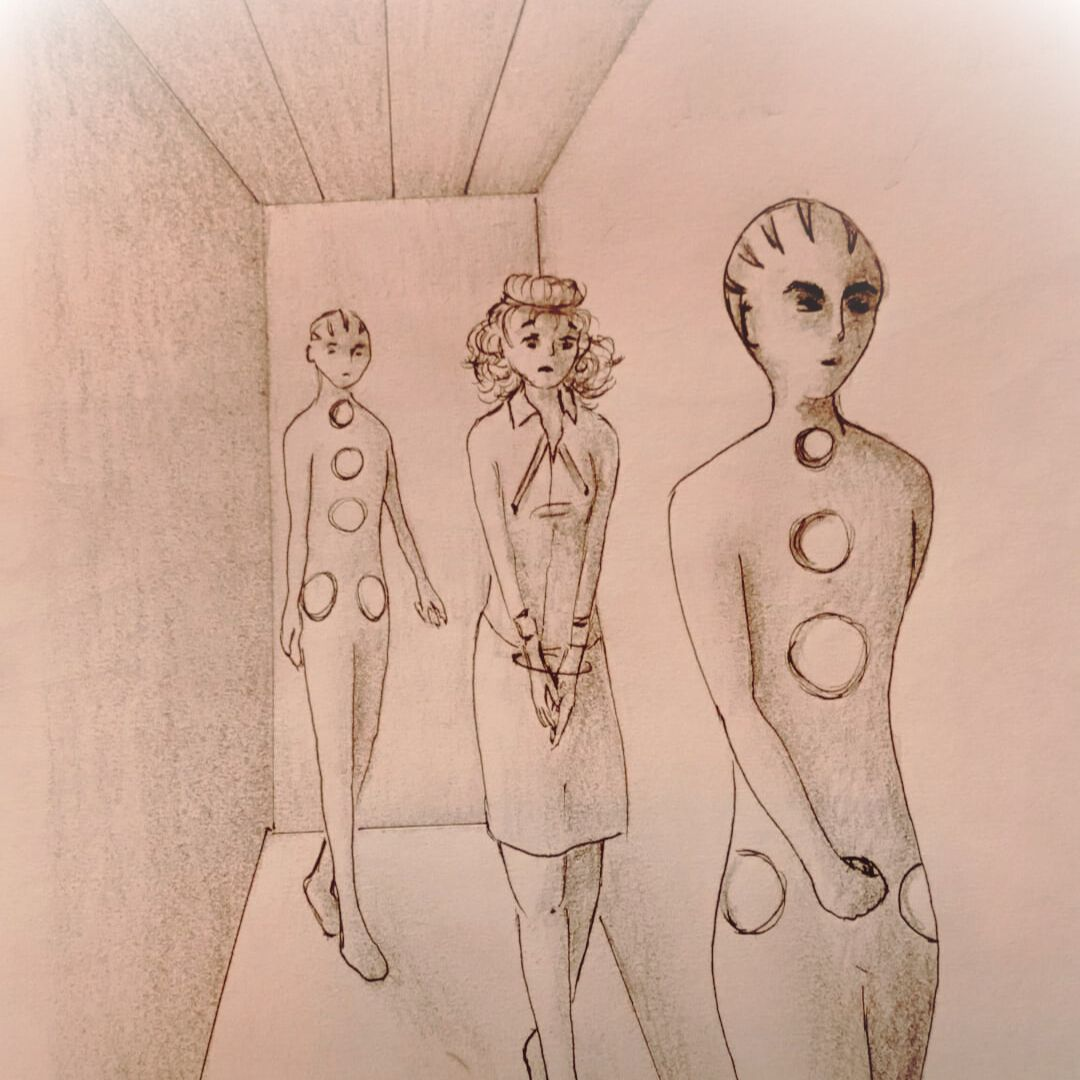
\includegraphics[width=\textwidth]{immagini/cnot_58.jpeg}} % Sostituisci con il nome del file immagine
\end{minipage}
\end{center}

\vspace{1em}
\begin{center}Caterina\end{center}
\hrule
\vspace{1em}

Mentre venivo scortata lungo corridoi freddi e squadrati, mi sentivo perduta. Il cuore mi batteva forte, non solo per la paura dell'ignoto, ma per qualcosa di più profondo che mi confondeva. Ripensai a come Mark si era alzato per difendermi, senza esitazione, e a come quella sicurezza e determinazione mi avessero dato una forza nuova, un senso di protezione che non avevo mai osato desiderare apertamente.

Mi resi conto, con una certa sorpresa, di quanto fosse importante per me sentirmi difesa, protetta da qualcuno capace di farsi avanti per me, di affrontare i pericoli con fermezza. Nella vita reale, non mi ero mai concessa di esprimere questo bisogno; con il mio fidanzato, avevo sempre mostrato una facciata forte e indipendente, temendo di sembrare fragile o insicura. Quante volte lui aveva cercato di esserci per me, di offrirmi un sostegno che, ora lo capivo, avevo rifiutato senza rendermi conto del danno che arrecavo a entrambi?

Mi sentivo vulnerabile, ma per la prima volta accettavo quel sentimento come parte di me, come un segnale che non dovevo soffocare. Mentre avanzavo verso il Commissario, capii che forse, una volta fuori, avrei dovuto riconsiderare il mio rapporto con il mio fidanzato, permettendogli di prendersi cura di me, vivendola non come una debolezza, ma come una connessione più autentica e reciproca.
